\documentclass[12pt]{article}
\newcommand{\bottomMargin}{2cm}

\newcommand{\header}{
	ДИЗАЙН И АНАЛИЗ НА АЛГОРИТМИ - \\ ПРАКТИКУМ\\
	\vspace{0.1cm}
        Летен семестър, 2025 г., домашно\\
	\vspace{0.1cm}
}
\newcommand{\tl}{$0,2$ сек.}
\newcommand{\ml}{$256$ MB}

%---DOCUMENT MARGINS---
\usepackage{geometry} % Required for adjusting page dimensions and margins
\geometry{
	paper=a4paper, % Paper size, change to letterpaper for US letter size
	top=4cm, % Top margin
	bottom=\bottomMargin, % Bottom margin
	left=2cm, % Left margin
	right=2cm, % Right margin
	headheight=3cm, % Header height
	%footskip=1.5cm, % Space from the bottom margin to the baseline of the footer
	headsep=0.5cm, % Space from the top margin to the baseline of the header
	%showframe, % Uncomment to show how the type block is set on the page
}
\usepackage{cmap}

\usepackage[T2A]{fontenc}
\usepackage[bulgarian]{babel}
\usepackage{fontspec}
\setmainfont{Times New Roman}
\setsansfont{Times New Roman}
\setmonofont{Courier New}
\usepackage[math-style=TeX]{unicode-math}
\setmathfont{Latin Modern Math}

\usepackage[nobottomtitles*]{titlesec}
\titleformat
{\section} % command
{\normalfont\fontsize{14}{14}\sffamily\bfseries} % format
{} % label
{0pt} % sep
{} % before-code
\titlespacing{\section}{0pt}{0em}{0em}
\usepackage[dvipsnames]{xcolor}
\titleformat
{\subsection} % command
{\fontsize{14}{14}\itshape} % format
{} % label
{0pt} % sep
{} % before-code
[\vspace{-1em}{\color{BrickRed}\rule{0.2\textwidth}{0.2em}}\vspace{-0.7em}] % after-code
\titlespacing{\subsection}{0pt}{0.5em}{0em}

\setlength{\parskip}{0.5em}
\setlength{\parindent}{24pt}
\sloppy

\usepackage{fancyhdr}
\pagestyle{fancy}
\usepackage{setspace}
\fancyhead[L]{
	\begin{minipage}{\textwidth}
		
\includegraphics[width=2.8cm]{/structure/logo.png}
	\end{minipage}
}
\fancyhead[C]{
	\begin{minipage}{\textwidth}
		\centering\large{\bf{\header}}
		\vspace{-0.35cm}
	\end{minipage}
}
\usepackage{emoji}
\usepackage{makecell}
\usepackage{tabularray}
\AtBeginEnvironment{table}{\vspace{-0.2cm}}
\AtEndEnvironment{table}{\vspace{-0.2cm}}
\usepackage{float}
\fancyhead[R]{
	\begin{tabular}{r@{\hspace{0.2cm}}l}
		\emoji{hourglass-not-done}: & \tl \\ 
		\emoji{floppy-disk}: & \ml \\ 
	\end{tabular}%
}
\renewcommand{\headrulewidth}{0cm}
\fancyheadoffset[L]{1cm}
\fancyheadoffset[R]{1cm}

\raggedbottom

\usepackage{amsmath}
\usepackage{stmaryrd}

\usepackage{graphicx}
\graphicspath{{./}}
\usepackage[export]{adjustbox}
\usepackage{wrapfig}
\makeatletter
\patchcmd\WF@putfigmaybe{\lower\intextsep}{}{}{\fail}
\AddToHook{env/wrapfigure/begin}{\setlength{\intextsep}{0pt}}
\makeatother
\usepackage[inkscapearea=page,inkscapepath=./svg-inkscape]{svg}
\svgpath{{./}}

\usepackage{placeins}
\usepackage{caption}
\captionsetup[table]{
	skip=0.25em,font=it,
	singlelinecheck=false,justification=justified,indention=-24pt,
	margin={24pt, 0pt}
}

\usepackage{enumitem}
\setlist{itemsep=-0.4em,leftmargin=\parindent,topsep=-\parskip}
\newcommand{\tabitem}{\indent~~\llap{\textbullet}~~}

\usepackage{hyperref}
\hypersetup{
	colorlinks=true,
	citecolor=blue,
	linkcolor=blue,
	urlcolor=cyan,
}


\begin{document}
\section{Задача H1. Ракети}
В един футуристичен град на име ``ФМИ`` има редица от $N$ небостъргачи, $i$-тия от тях с широчина $w_i$ и височина $h_i$. Те са построени един до друг, без никакви празнини между тях и без да се застъпват.

Вие сте участвате в отряд, който изстрелва ракети срещу града. Отрядът смята да изстреля $M$ на брой ракети, като планът е $i$-тата ракета да прелети на широчина $x_i$ и височина $y_i$ (считаме, че нулевата широчина е тази, в която започва първата сграда).

Напишете програма \textbf{\texttt{rockets}}, която намира колко ракети ще ударят поне един небостъргач.
\subsection{Вход}
От първия ред на стандартния вход се въвеждат две цели числа n и m – брой на небостъргачите и брой на ракетите. От следващите n реда се въвеждат по две цели числа $w_i$ и $h_i$ – широчината и височината на $i$-тия небостъргач. От следващите m реда се въвеждат по две цели числа $x_j$ и $y_j$ – широчина и височина на $j$-тата ракета

\subsection{Изход}
На първия ред на стандартния изход изведете едно цяло число – броя ракети, които ще ударят поне един небостъргач.

\subsection{Ограничения}
\begin{itemize}
	\item $1\leq N, M \leq 300\ 000$
    \item $1\leq h_i, w_i \leq 10^9$
    \item $1\leq x_i, y_i \leq 10^9$
    %\item В ??? процента от тестовете $1\leq N, M \leq 10^3$
\end{itemize}

\subsection{Пример}
\begin{table}[H]
	\begin{tblr}{|X[12,l]|X[8,l]|X[80,j]|}
		\hline
		\textbf{Вход} & \textbf{Изход} & \textbf{Обяснение на примера} \\
		\hline
		\texttt{4 8  \\
2 3 \\
3 6 \\
2 4 \\
4 2 \\
1 2 \\
3 7 \\
4 2 \\
5 8 \\
7 4 \\
9 1 \\
9 5 \\
12 8 \\
}
		& 
		\texttt{4}
		& 
		{На фигурата е показано разположението на небостъргачите и ракетите. \\
        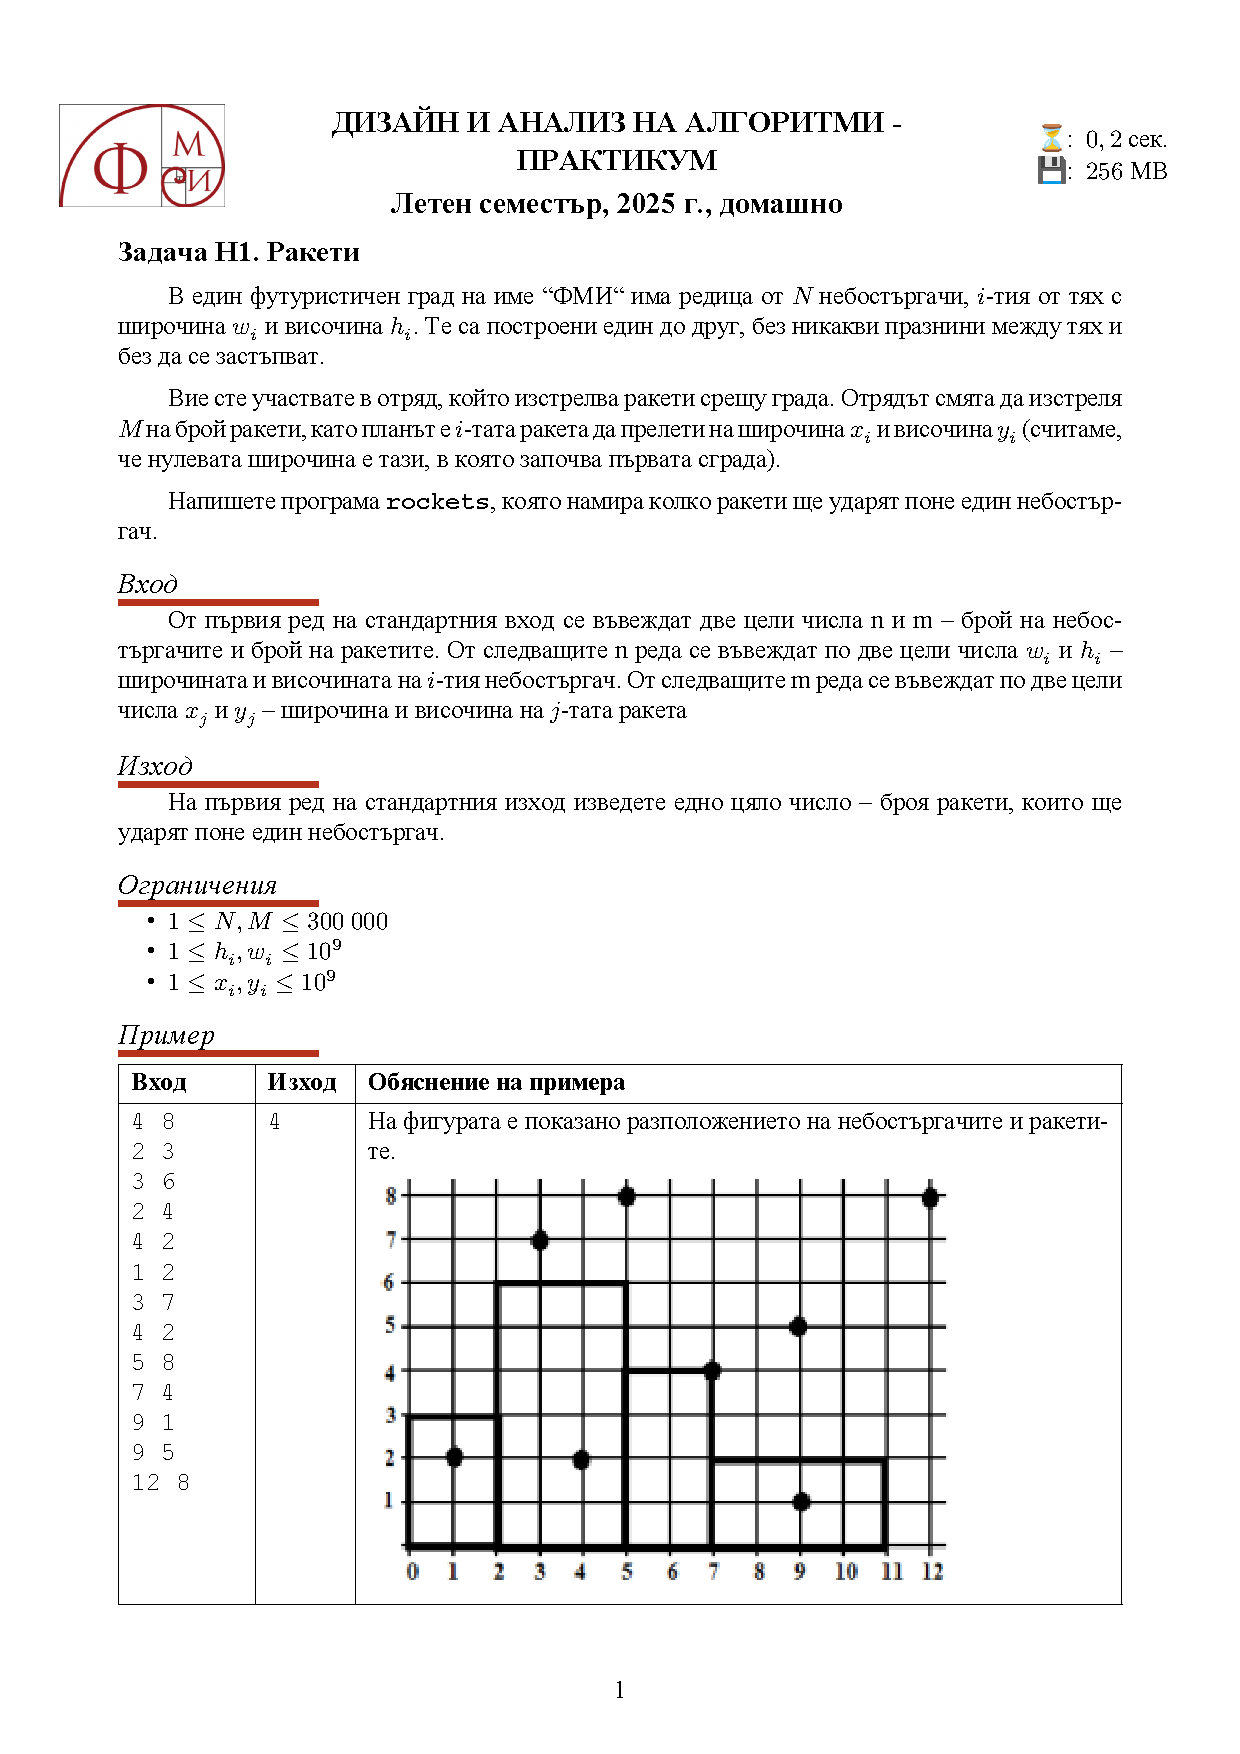
\includegraphics[width = 10cm]{rockets.png}
        } \\
		\hline
	\end{tblr} 
\end{table}
\FloatBarrier

\end{document}
